
\subsection{Rejestracja konta użytkownika}
Funkcjonalność umożliwiająca rejestrację w aplikacji.

\subsubsection{Backend}
Po wysłaniu requesta na przez aplikacje webową lub mobilną api wyciąga przesłane dane, weryfikuje je. Do weryfikacji należy:

\begin{itemize}
    \item Czy użytkownik z wprowadzonym e-mail istnieje już w bazie;
    \item Czy użytkownik z wprowadzoną nazwą użytkownika istnieje już w bazie;
    \item Czy przesłane hasła są równe.
\end{itemize}

W przypadku błędnej weryfikacji zwraca odpowiednią wiadomość z błędem dla użytkownika np. "Wprowadzony e-mail jest już zajęty". Natomiast jeśli weryfikacja przebiegnie pomyślnie, użytkownik zostanie dodany do bazy, a system wyśle mu wiadomość e-mail z prośbą o aktywację konta.

\begin{figure}[H]
    \centering
    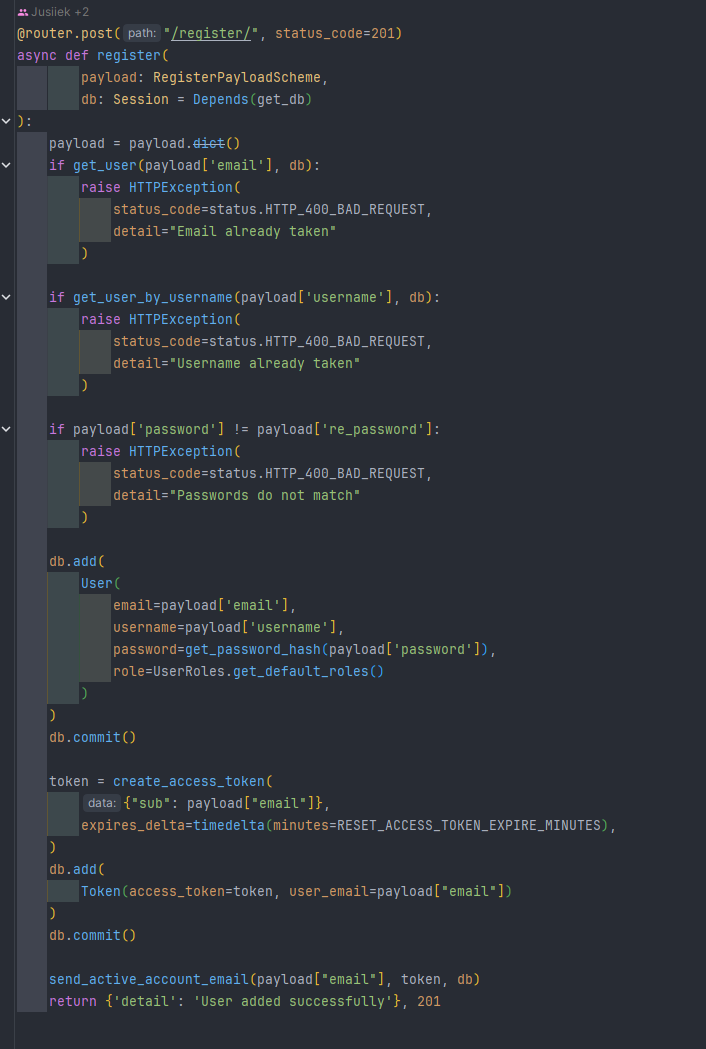
\includegraphics[width=0.7\textwidth]{chapters/chapter_8/screens/rejestracja_backend}
    \caption{Implementacja kodu rejestracji użytkownika w backendzie.}
    \label{img:rejestracja_backend}
\end{figure}

\subsubsection{Aplikacja moblina i aplikacja webowa}
Aby założyć konto, użytkownik musi wypełnić formularz rejestracyjny wymagający podania nazwy użytkownika, adresu e-mail oraz hasła wpisanego jednakowego do dwóch pól w celach jego walidacji. Aplikacja pozwoli na utworzenie konta jedynie jeżeli:

\begin{itemize}
    \item Pseudonim zawiera od 3 do 20 znaków i składa się wyłącznie z liter, cyfr, lub podkreślników;
    \item Adres e-mail jest dostarczony w prawidłowym dla niego formacie;
    \item Hasło posiada co najmniej 8 znaków;
    \item Hasło wpisane oba pola walidacyjne jest w nich takie samo;
    \item Adres e-mail i nazwa użytkownika są unikalne (czyli w bazie danych nie są przypisane do żadnego innego konta).
\end{itemize}

Po zatwierdzeniu prawidłowych danych aplikacja informuje komunikatem o udanym utworzeniu konta. Użytkownik zostaje przeniesiony do strony logowania. W przypadku podania nieprawidłowych danych, użytkownik nie zostanie zarejestrowany i zostanie powiadomiony komunikatem w aplikacji o błędzie.

\begin{figure}[H]
    \centering
    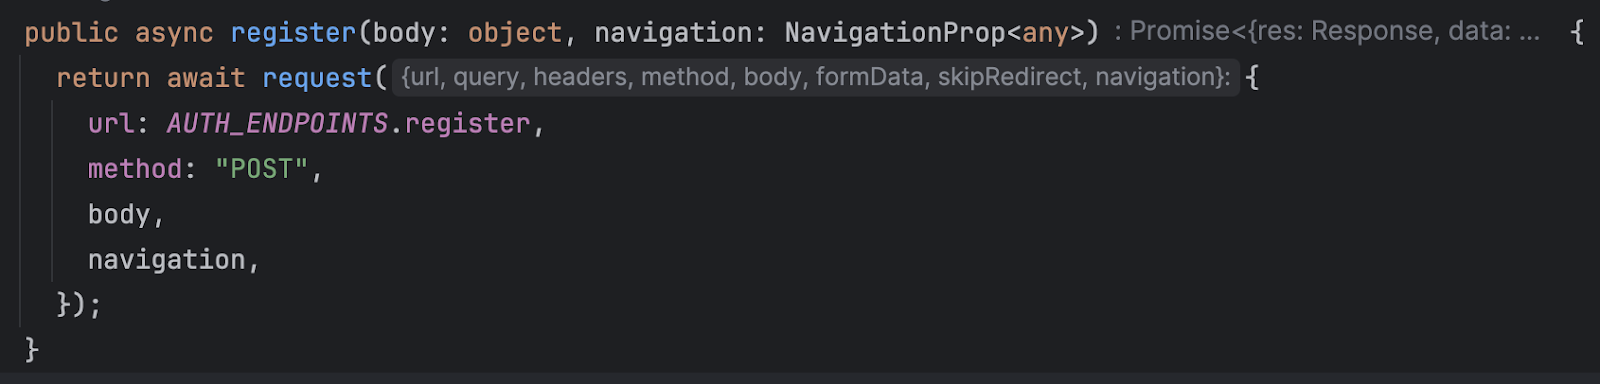
\includegraphics[width=0.7\textwidth]{chapters/chapter_8/screens/rejestracja_mobile}
    \caption{Metoda "register" w serwisie Auth zastosowana w aplikacji mobilnej.}
    \label{img:rejestracja_mobile}
\end{figure}

\begin{figure}[H]
    \centering
    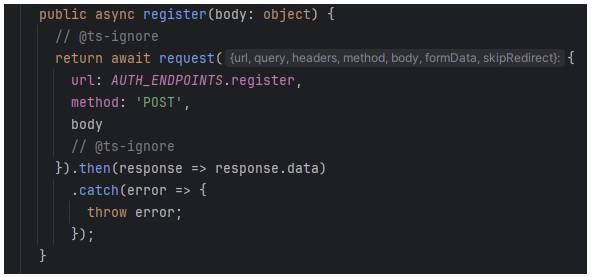
\includegraphics[width=0.7\textwidth]{chapters/chapter_8/screens/rejestracja_web}
    \caption{Metoda "register" w serwisie AuthService zastosowana w aplikacji webowej.}
    \label{img:rejestracja_web}
\end{figure}

Powyższe funkcję wysyłają asynchroniczne żądanie POST do serwera w celu rejestracji nowego użytkownika. Metoda przekazuje dane rejestracyjne w treści żądania, a następnie zwraca czy żądanie zostało obsłużone.

\subsection{Logowanie do systemu}
Funkcjonalność umożliwiająca logowanie do aplikacji

\subsubsection{Backend}
Po wysłaniu requesta na przez aplikację webową lub mobilną api wyciąga przesłane dane, weryfikuje je.
Weryfikacja odbywa się za pomocą funkcji \texttt{authenticate\_user} zaimportowaną z utils’ów.
Ta najpierw próbuje wyciągnąć z użytkownika z bazy, który posiada wysłany e-mail. Potem, jeżeli użytkownik istnieje, sprawdzamy hasło metodą klasową \texttt{verify\_password}. Jeśli wszystko przebiegło pomyślnie, użytkownikowi zostanie zwrócony token autoryzacji i dane użytkownika. W przeciwnym razie zwrócona wiadomość i błędnie wprowadzonych danych.

\begin{figure}[H]
    \centering
    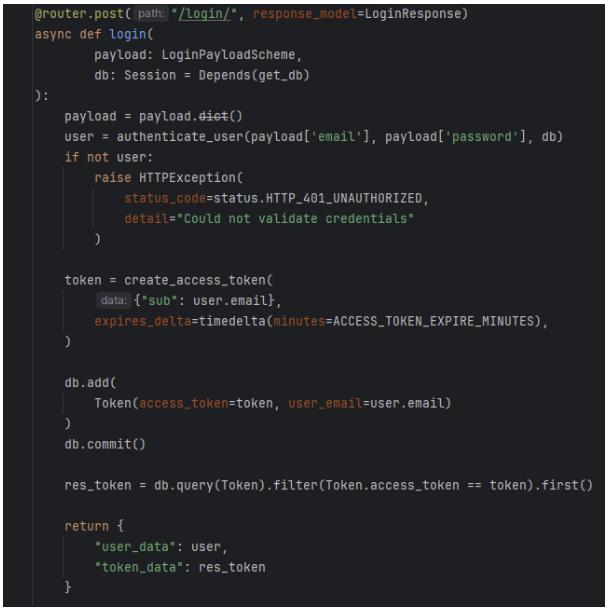
\includegraphics[width=0.7\textwidth]{chapters/chapter_8/screens/logowanie_backend}
    \caption{Implementacja kodu logowania użytkownika w backendzie.}
    \label{img:logowanie_backend}
\end{figure}

\subsubsection{Aplikacja mobilna i aplikacja webowa}
Na stronie logowania, użytkownik musi wypełnić formularz wymagający uzupełnienia pól adres e-mail oraz hasło. Po zatwierdzeniu danych i ich weryfikacji pojawia się komunikat o zalogowaniu użytkownika, a następnie użytkownik zostanie przeniesiony na stronę główną. W przypadku podania nieprawidłowych danych, użytkownik nie zostanie zalogowany i zostanie poinformowany komunikatem o błędzie.

\begin{figure}[H]
    \centering
    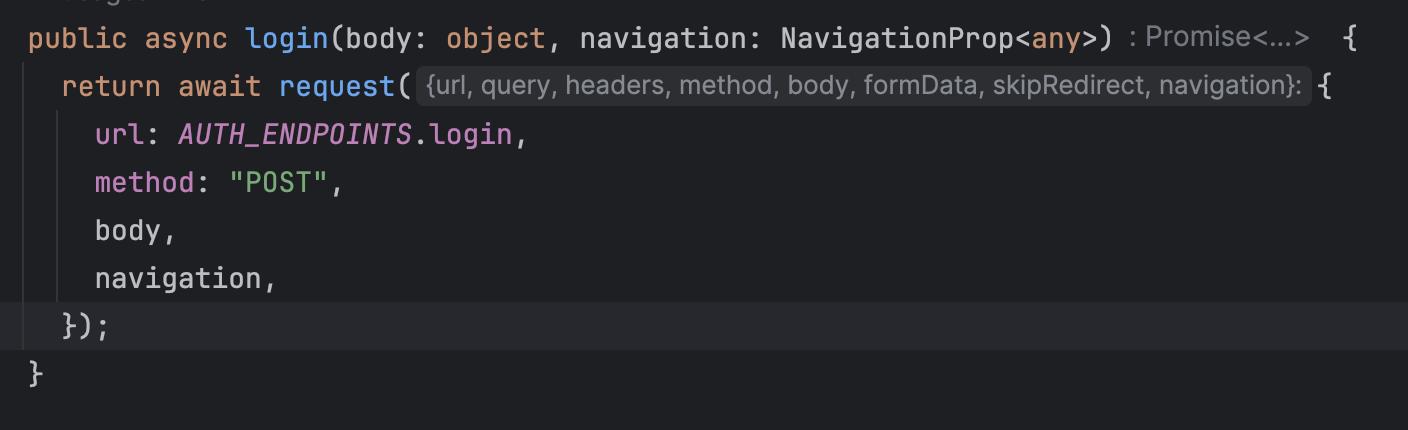
\includegraphics[width=0.7\textwidth]{chapters/chapter_8/screens/logowanie_mobile}
    \caption{Metoda "login" zastosowana w aplikacji mobilnej.}
    \label{img:logowanie_mobile}
\end{figure}

\begin{figure}[H]
    \centering
    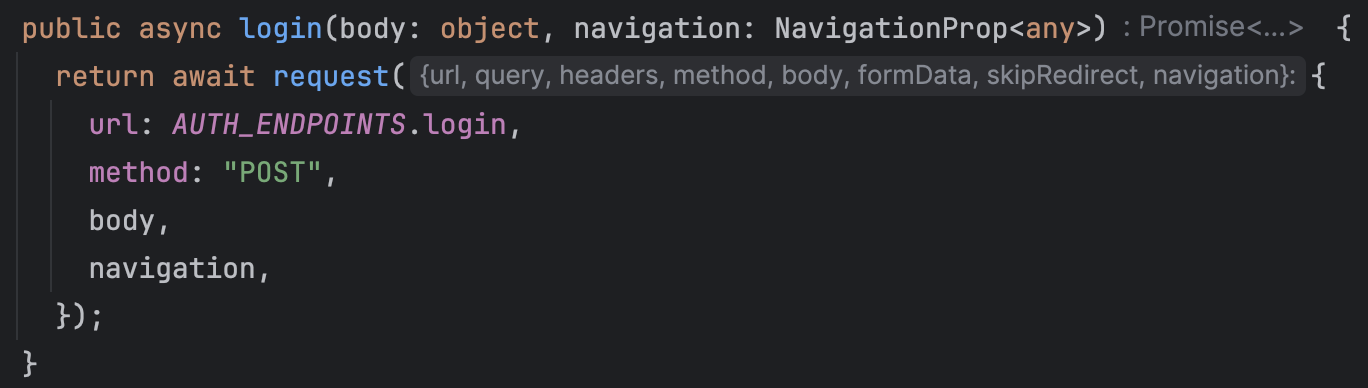
\includegraphics[width=0.7\textwidth]{chapters/chapter_8/screens/logowanie_web}
    \caption{Metoda "login" zastosowana w aplikacji webowej.}
    \label{img:logowanie_web}
\end{figure}

Użyta w powyższych metodach funkcja \texttt{ActiveUser.set(data)} zapisuje dane zalogowanego użytkownika w lokalnym stanie aplikacji. Dzięki temu, informacje o użytkowniku, takie jak token autoryzacyjny, mogą być łatwo dostępne w całej aplikacji. Pozwala to na:

\begin{itemize}
    \item Personalizację interfejsu użytkownika (np. wyświetlanie nazwy użytkownika);
    \item Umożliwienie dostępu do zasobów, które wymagają uwierzytelnienia;
    \item Przechowywanie sesji użytkownika, aby mógł pozostać zalogowany pomiędzy różnymi wizytami na stronie.
\end{itemize}

\subsection{Wylogowanie z systemu}
Funkcjonalność pozwalająca na wylogowanie użytkownika.

\subsubsection{Backend}
Po kliknięciu wyloguj w aplikacji mobilnej czy w webowej, zostaje wysłany request na api, który dodaje aktualnie używany token do listy nieaktualnych tokenów.

\begin{figure}[H]
    \centering
    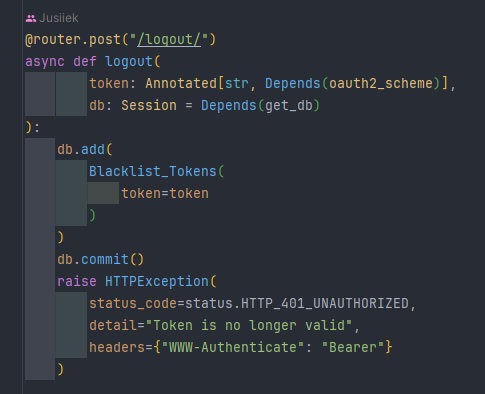
\includegraphics[width=0.7\textwidth]{chapters/chapter_8/screens/wylogowanie_backend}
    \caption{Implementacja kodu wylogowania użytkownika w backendzie.}
    \label{img:wylogowanie_backend}
\end{figure}

\subsubsection{Aplikacja mobilna i aplikacja webowa}
Aby wylogować się z aplikacji, użytkownik musi kliknąć w nawigacji "Logout". Po kliknięciu przycisku, dane użytkownika zostaną usunięte z pamięci lokalnej. Token autoryzacyjny użytkownika utworzony przy logowaniu zostanie dodany w bazie danych do tabeli zawierającej nieaktywne tokeny.

\begin{figure}[H]
    \centering
    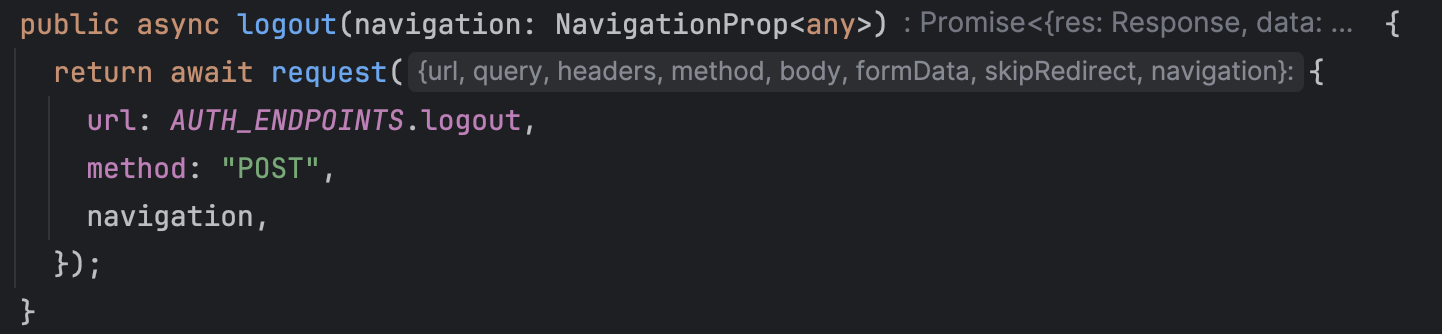
\includegraphics[width=0.7\textwidth]{chapters/chapter_8/screens/wylogowanie_mobile}
    \caption{Metoda "logout" zastosowana w aplikacji mobilnej.}
    \label{img:wylogowanie_mobile}
\end{figure}

\begin{figure}[H]
    \centering
    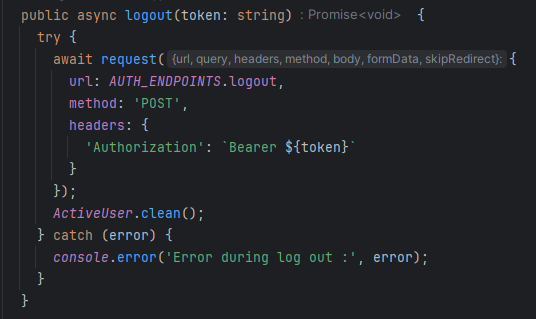
\includegraphics[width=0.7\textwidth]{chapters/chapter_8/screens/wylogowanie_web}
    \caption{Metoda "logout" zastosowana w aplikacji webowej.}
    \label{img:wylogowanie_web}
\end{figure}

Powyższe fragmenty serwisu odpowiadają za usunięcie danych użytkownika z pamięci lokalnej wykorzystujący endpoint dezaktywujący token autoryzacji.

\subsection{Edycja danych użytkownika}
Funkcjonalność umożliwiająca edycję danych użytkownika.

\subsubsection{Backend}
Aplikacje frontendowe wysyłają dane do aktualizacji np. e-mail. Jedynym obowiązkowym atrybutem przy aktualizacji jest \texttt{current\_password}. Po zweryfikowaniu zgodności hasła, system przystępuje do zmiany danych wprowadzonych przez użytkownika. Na koniec zostają zwrócone użytkownika z poprawionym polami.

\begin{figure}[H]
    \centering
    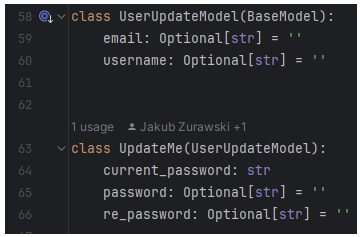
\includegraphics[width=0.5\textwidth]{chapters/chapter_8/screens/edit_user_backend_1}
    \caption{Implementacja klas modeli "UserUpdateModel" i "UpdateMe" w backendzie.}
    \label{img:edit_user_backend_1}
\end{figure}

\begin{figure}[H]
    \centering
    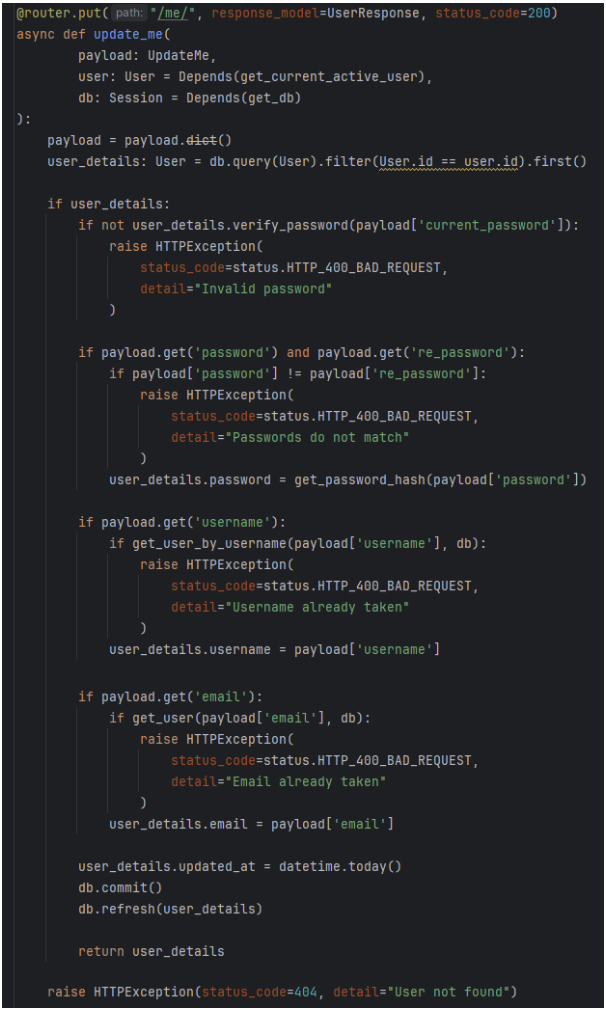
\includegraphics[width=0.7\textwidth]{chapters/chapter_8/screens/edit_user_backend_2}
    \caption{Implementacja kodu zmiany danych użytkownika w backendzie.}
    \label{img:edit_user_backend_2}
\end{figure}

\subsubsection{Aplikacja mobilna i aplikacja webowa}
W celu zmiany danych użytkownika, takich jak avatar, nazwa użytkownika, adres e-mail czy hasło, użytkownik może skorzystać z odpowiednich formularzy dostępnych na stronie profilu użytkownika. Każda zmiana (za wyjątkiem zmiany avatara) wymaga uwierzytelnienia przez podanie aktualnego hasła. Poniżej opisane są poszczególne procesy.

\begin{figure}[H]
    \centering
    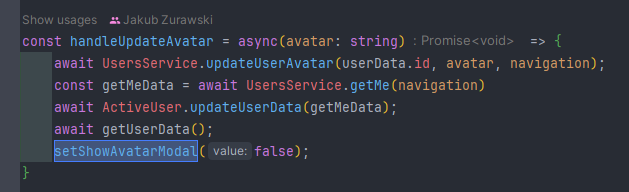
\includegraphics[width=0.7\textwidth]{chapters/chapter_8/screens/edit_user_mobile}
    \caption{Funkcja "handleAvatarSelect" zastosowany w aplikacji mobilnej.}
    \label{img:edit_user_mobile}
\end{figure}

\begin{figure}[H]
    \centering
    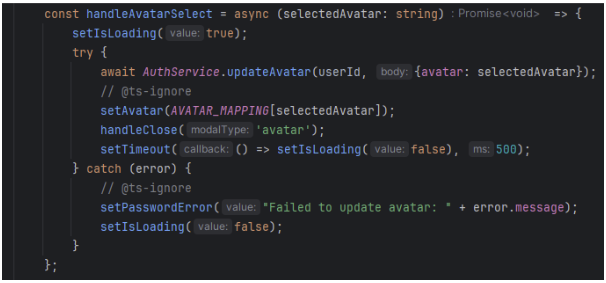
\includegraphics[width=0.7\textwidth]{chapters/chapter_8/screens/edit_user_web}
    \caption{Funkcja "handleAvatarSelect" zastosowany w aplikacji webowej.}
    \label{img:edit_user_web}
\end{figure}

\textbf{Zmiana avatara}\\
Aby zmienić avatar, użytkownik musi wybrać nowy avatar z dostępnych opcji. Po dokonaniu wyboru aplikacja wysyła żądanie do serwera w celu aktualizacji avatara. Po pomyślnej aktualizacji użytkownik zobaczy nowy avatar na stronie profilu oraz w widoku statystyk.\\


\textbf{Zmiana pseudonimu}\\
Aby zmienić pseudonim, użytkownik musi wprowadzić nowy pseudonim oraz aktualne hasło w odpowiednim formularzu. Po zatwierdzeniu formularza dane są walidowane:
\begin{itemize}
    \item Pseudonim musi zawierać 3-20 znaków i składać się wyłącznie z liter, cyfr lub podkreślników;
    \item Aktualne hasło musi być poprawne.
\end{itemize}
Jeśli dane są poprawne, aplikacja wysyła żądanie do serwera w celu aktualizacji pseudonimu. Po pomyślnej aktualizacji nowy pseudonim będzie wyświetlany na stronie profilu.\\


\textbf{Zmiana adresu e-mail}\\
Aby zmienić adres e-mail, użytkownik musi wprowadzić nowy adres e-mail oraz aktualne hasło w odpowiednim formularzu. Po zatwierdzeniu formularza dane są walidowane:
\begin{itemize}
    \item Adres e-mail musi mieć poprawny format;
    \item Aktualne hasło musi być poprawne.
\end{itemize}
Jeśli dane są poprawne, aplikacja wysyła żądanie do serwera w celu aktualizacji adresu e-mail. Po pomyślnej aktualizacji użytkownik będzie logował się nowym adresem e-mail.\\


\textbf{Zmiana hasła}\\
Aby zmienić hasło, użytkownik musi wprowadzić aktualne hasło, nowe hasło oraz potwierdzenie nowego hasła w odpowiednim formularzu. Po zatwierdzeniu formularza dane są walidowane:
\begin{itemize}
    \item Nowe hasło musi mieć co najmniej 8 znaków;
    \item Potwierdzenie nowego hasła musi być zgodne z nowym hasłem;
    \item Aktualne hasło musi być poprawne.
\end{itemize}
Jeśli dane są poprawne, aplikacja wysyła żądanie do serwera w celu aktualizacji hasła.

\subsection{Usunięcie konta użytkownika}
Funkcjonalność umożliwiająca usunięcie konta użytkownika.

\subsubsection{Backend}
Aplikacje frontendowe wysyłają na api e-mail użytkownika i hasło. Api sprawdza poprawność danych, następnie usuwa konto użytkownika.

\begin{figure}[H]
    \centering
    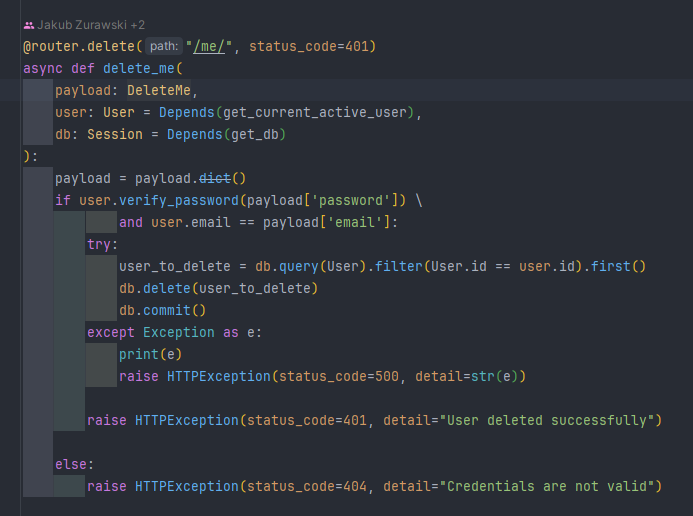
\includegraphics[width=0.7\textwidth]{chapters/chapter_8/screens/delete_user_backend}
    \caption{Implementacja kodu usunięcia użytkownika w backendzie.}
    \label{img:delete_user_backend}
\end{figure}

\subsubsection{Aplikacja moblina}
Użytkownik jest proszony o potwierdzenie czy aby na pewno chce usunąć konto. Po zatwierdzeniu zostaje przekierowany do formularza gdzie podaje e-mail oraz hasło, które po zatwierdzeniu zostają wysłane na api.

\begin{figure}[H]
    \centering
    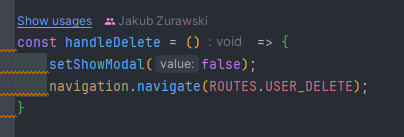
\includegraphics[width=0.7\textwidth]{chapters/chapter_8/screens/delete_user_mobile_1}
    \caption{Wywołanie funkcji "handleDelete" zastosowanego w aplikacji mobilnej.}
    \label{img:delete_user_mobile_1}
\end{figure}

\begin{figure}[H]
    \centering
    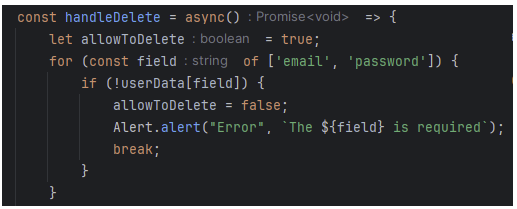
\includegraphics[width=0.7\textwidth]{chapters/chapter_8/screens/delete_user_mobile_2}
    \caption{Funkcja "handleDelete" zastosowany w aplikacji mobilnej.}
    \label{img:delete_user_mobile_2}
\end{figure}

\subsubsection{Aplikacja webowa}

Jeżeli po potwierdzeniu wyboru prawidłowym hasłem, funkcja wykryje błąd "error 401 (Unauthorized)", oznaczać to będzie że konto zostało usunięte. Następnie pojawia się komunikat o usunięciu który przekierowuje do strony logowania

\begin{figure}[H]
    \centering
    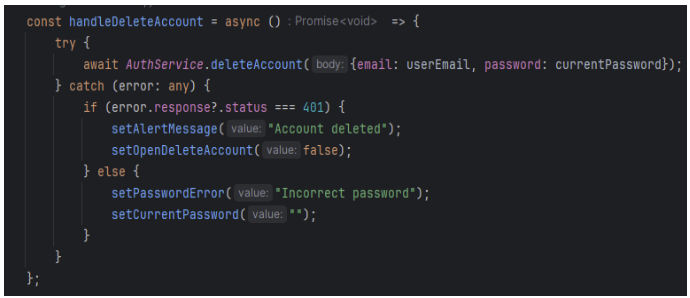
\includegraphics[width=0.7\textwidth]{chapters/chapter_8/screens/delete_user_web}
    \caption{Funkcja "handleDelete" zastosowany w aplikacji webowej.}
    \label{img:delete_user_web}
\end{figure}

\subsection{Tworzenie talii fiszek}

Funkcjonalność umożliwiająca tworzenie talii fiszek.

\subsubsection{Backend}

Utworzono metodę POST, która umożliwia tworzenie talii o podanej nazwie i kategorii. Do tworzenia fiszki używana jest osobna metoda POST, która przyjmuje treść dla przedniej i tylnej strony karty, a także identyfikator talii do, której utworzona fiszka zostanie przypisana.

\begin{figure}[H]
    \centering
    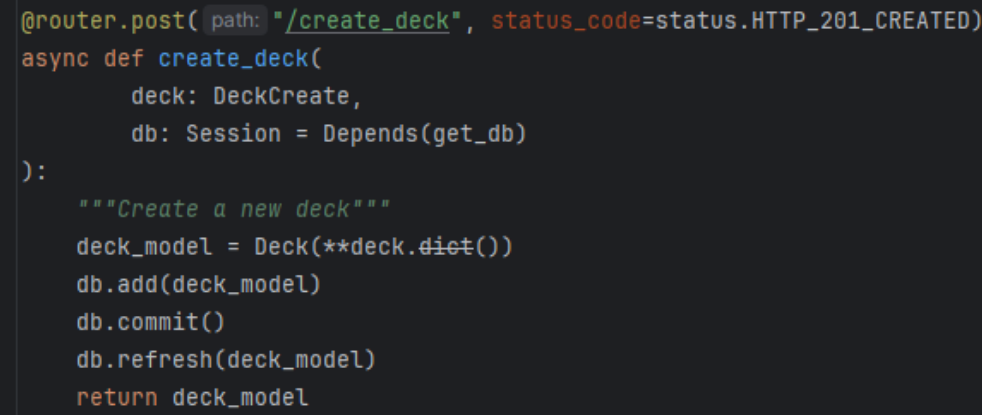
\includegraphics[width=0.7\textwidth]{chapters/chapter_8/screens/create_deck_backend}
    \caption{Logika tworzenia decku po stronie serwera.}
    \label{img:create_deck_backend}
\end{figure}

\begin{figure}[H]
    \centering
    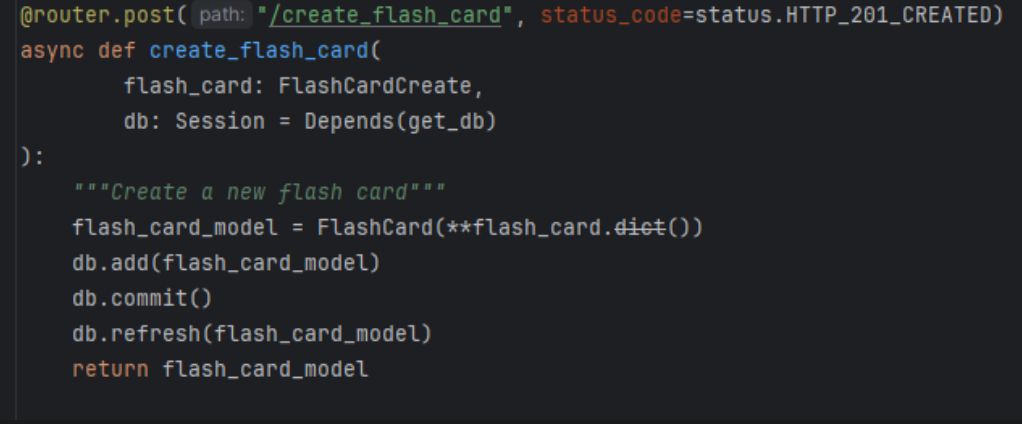
\includegraphics[width=0.7\textwidth]{chapters/chapter_8/screens/create_flash_card_backend}
    \caption{Logika tworzenia fiszek po stronie serwera.}
    \label{img:create_flash_card_backend}
\end{figure}

\subsubsection{Aplikacja mobilna}
Dodanie fiszki jest możliwe po przejściu do widoku jej tworzenia z podglądu wybranej talii. Wymagane jest uzupełnienie pól przedniej i tylnej strony fiszki. Tworzenie odbywa się przez wysłanie danych do odpowiedniego endpointu.

\begin{figure}[H]
    \centering
    \includegraphics[width=0.7\textwidth]{chapters/chapter_8/screens/create_deck_mobile}
    \caption{Funkcja obsługująca tworzenie nowej fiszki.}
    \label{img:create_deck_mobile}
\end{figure}

\subsubsection{Aplikacja webowa}

Użytkownik aby utworzyć talię musi wypełnić pole tekstowe dla nazwy i kategorii talii, następnie musi uzupełnić treść dla przedniej i tylnej strony fiszki. Po kliknięciu "Create deck" dane z formularzy zostają przekazane do funkcji, która zebrane dane przekazuje do serwisu odpowiedzialnego za komunikację z endpointem do tworzenia talii i endpointem do tworzenia fiszki.

\begin{figure}[H]
    \centering
    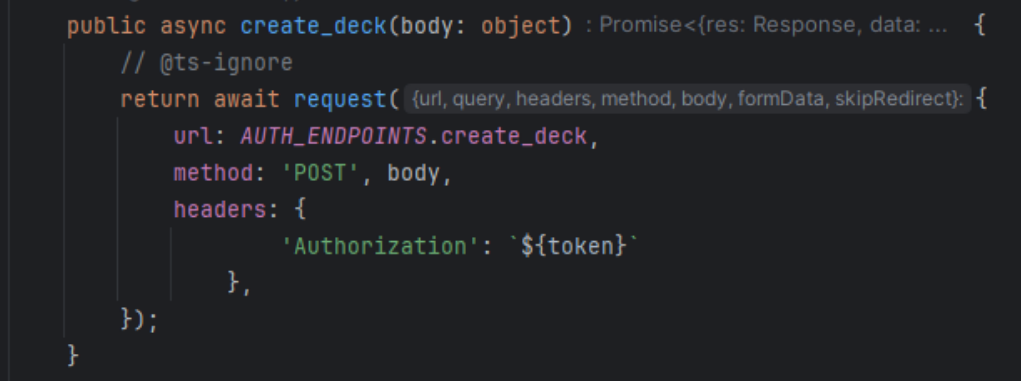
\includegraphics[width=0.7\textwidth]{chapters/chapter_8/screens/create_deck_web}
    \caption{Funkcja odpowiedzialna za komunikację z endpointem do tworzenia decku.}
    \label{img:create_deck_web}
\end{figure}

\begin{figure}[H]
    \centering
    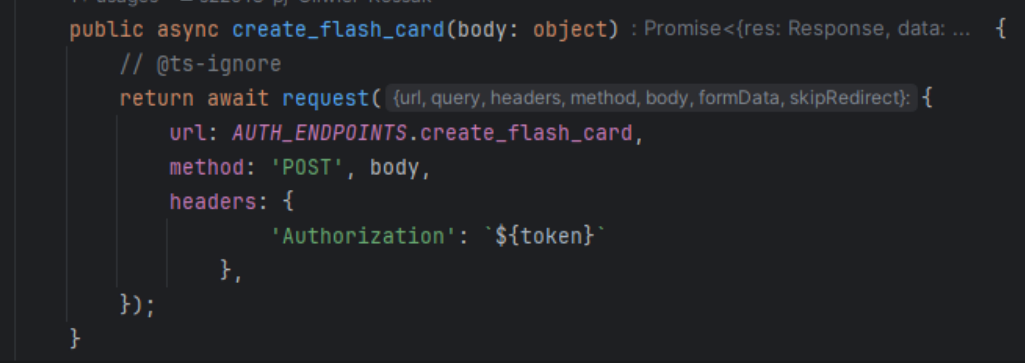
\includegraphics[width=0.7\textwidth]{chapters/chapter_8/screens/create_flash_card_web}
    \caption{Funkcja serwisu odpowiedzialna za komunikację z endpointem do tworzenia fiszki.}
    \label{img:create_flash_card_web}
\end{figure}

\subsection{Usunięcie talii fiszek}

Funkcjonalność umożliwiająca usunięcie talii fiszek.

\subsubsection{Backend}

Został utworzony endpoint \texttt{delete\_deck}, która pozwala na usunięcie talii o podanym identyfikatorze wraz z wszystkimi powiązanymi fiszkami.

\begin{figure}[H]
    \centering
    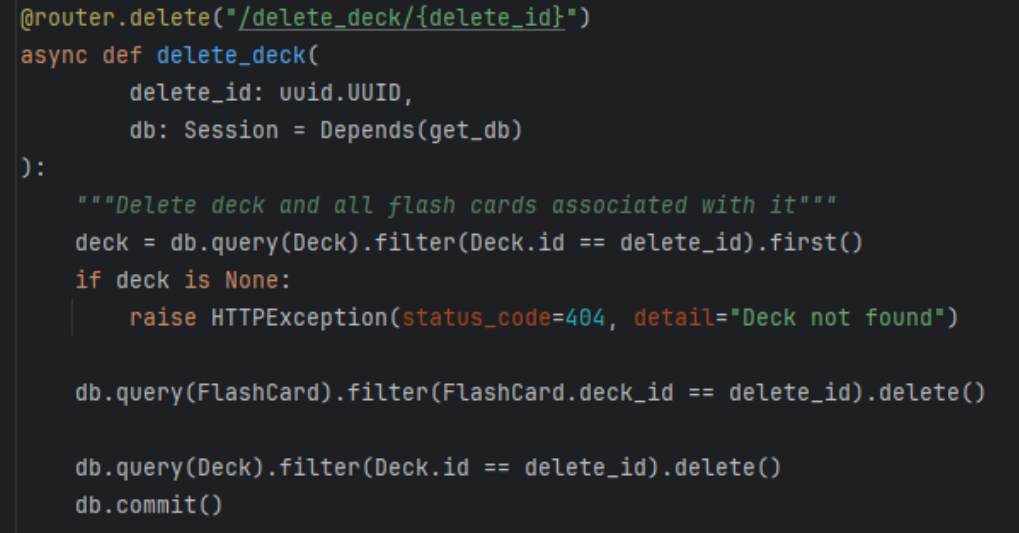
\includegraphics[width=0.7\textwidth]{chapters/chapter_8/screens/delete_deck_backend}
    \caption{Logika usuwająca talie i wszystkie należące do niej fiszki.}
    \label{img:delete_deck_backend}
\end{figure}


\subsubsection{Aplikacja moblina}
Usunięcie talii jest możliwe z poziomu jej opcji. Po wybraniu tej opcji do api zostaje wysłane zapytanie o usunięcie talii. W zapytaniu przekazywany jest jej identyfikator.

\begin{figure}[H]
    \centering
    \includegraphics[width=0.7\textwidth]{chapters/chapter_8/screens/delete_deck_mobile}
    \caption{Funkcja odpowiedzialna za obsługę usunięcia decku.}
    \label{img:delete_deck_mobile}
\end{figure}

\subsubsection{Aplikacja webowa}

Użytkownik aby usunąć talię klika w opcje, następnie wybiera "Delete deck". Po kliknięciu, identyfikator aktualnej talii zostaje pobrany z pamięci lokalnej i przekazane do serwisu, który łączy się z bakcendowym endpointem do usuwania talii. Endpoint usuwa z bazy danych talię o podanym identyfikatorze i wszystkie należące do niego fiszki.

\begin{figure}[H]
    \centering
    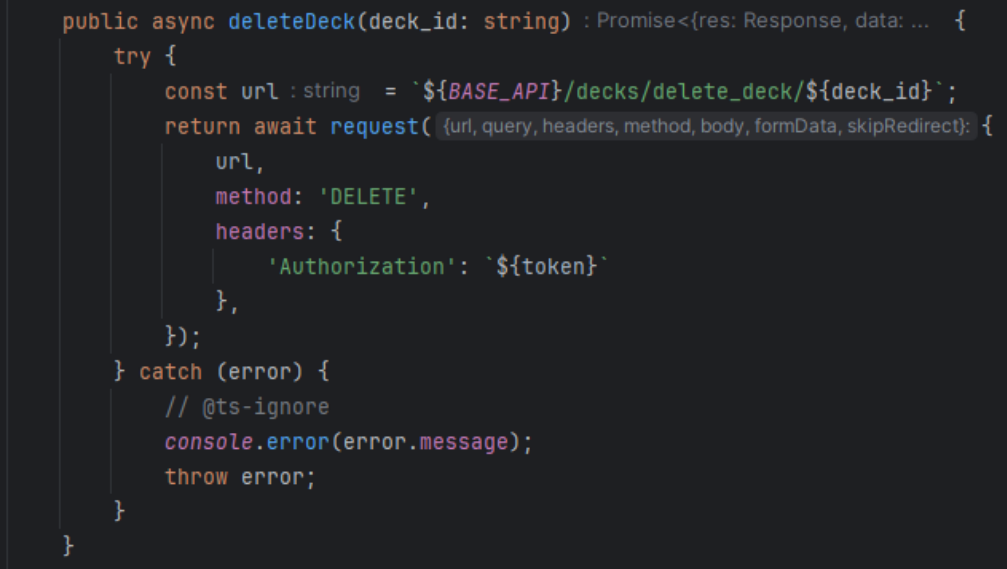
\includegraphics[width=0.7\textwidth]{chapters/chapter_8/screens/delete_deck_web}
    \caption{Funkcja serwisu odpowiedzialna za komunikację z endpointem do usuwania talii.}
    \label{img:delete_deck_web}
\end{figure}

\subsection{Edycja talii fiszek}

Funkcjonalność umożliwiająca aktualizowanie zawartości talii fiszek.

\subsubsection{Backend}

Zostały utworzone metody PUT, pozwalające na komunikację z bazą danych w celu aktualizacji informacji o fiszkach i taliach.

\begin{figure}[H]
    \centering
    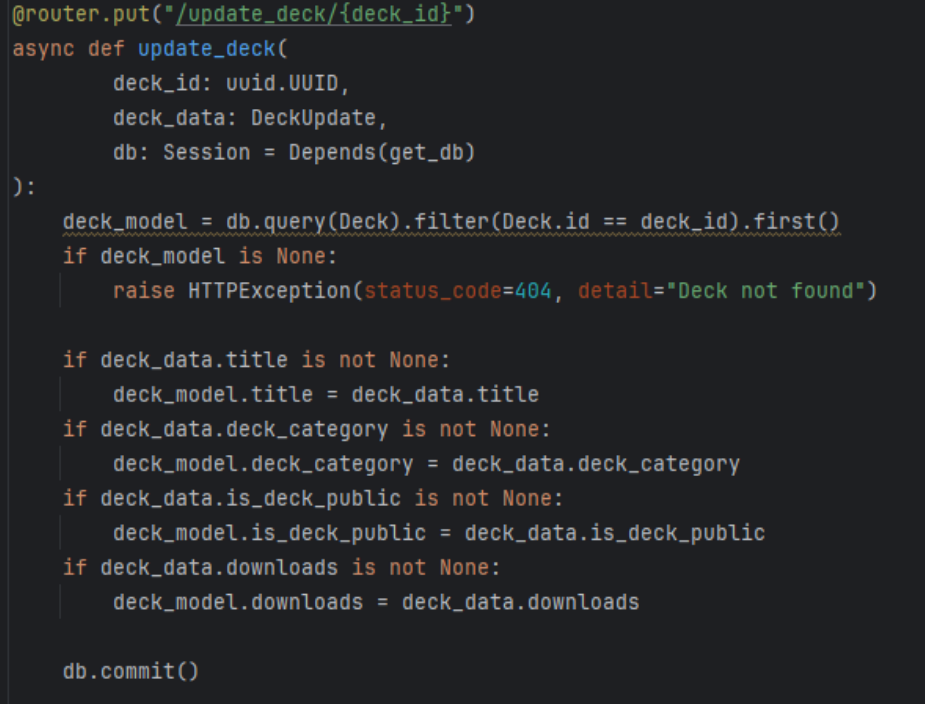
\includegraphics[width=0.7\textwidth]{chapters/chapter_8/screens/update_deck_backend}
    \caption{Metoda aktualizujące dane talii o podanym identyfikatorze.}
    \label{img:update_deck_backend}
\end{figure}

\begin{figure}[H]
    \centering
    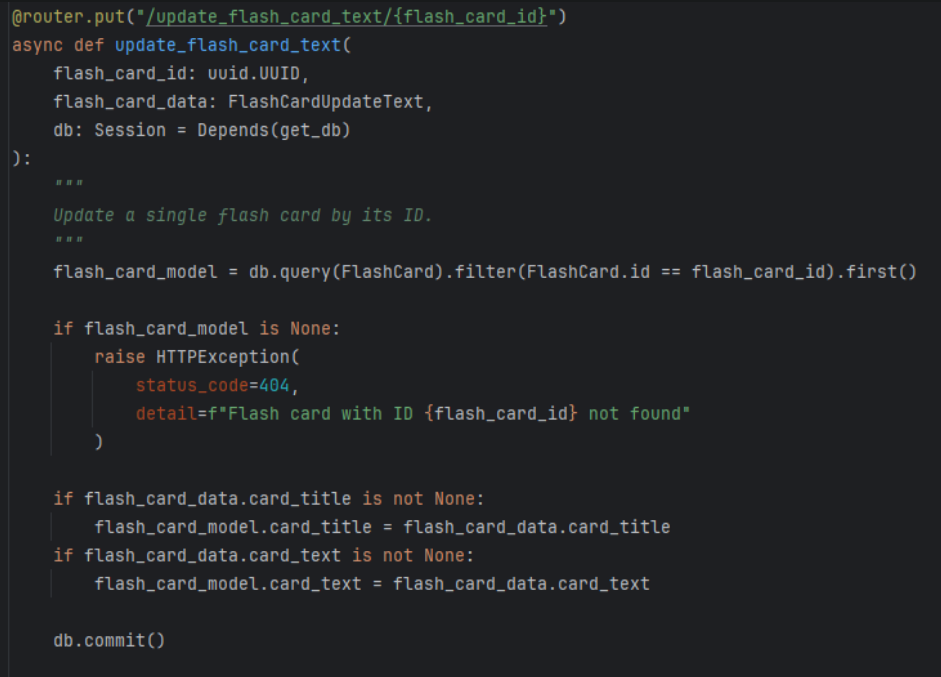
\includegraphics[width=0.7\textwidth]{chapters/chapter_8/screens/update_flash_card_text_backend}
    \caption{Metoda PUT aktualizująca dane fiszk.}
    \label{img:update_flash_card_backend}
\end{figure}

\subsubsection{Aplikacja moblina}

Aby zmienić nazwę lub kategorię talii, użytkownik musi wybrać widok "Edit" w jej opcjach. Aktualizacja danych odbywa się za zmianą treści pól "nazwa" i "kategoria" po zaakceptowaniu zmian, te wysyłane są na endpoint.

\begin{figure}[H]
    \centering
    \includegraphics[width=0.7\textwidth]{chapters/chapter_8/screens/update_deck_mobile}
    \caption{Funkcja obsługująca aktualizację danych talii.}
    \label{img:update_deck_mobile}
\end{figure}

\subsubsection{Aplikacja webowa}

Użytkownik w celu zmiany nazwy talii lub kategorii musi otworzyć okno opcji następnie klika w przycisk zmiany danych. Po wykonanie tych operacji pojawia się formularz do zmiany nazwy talii i kategorii. Użytkownik może podać nowe dane i kliknąć przycisk "Accept". Nowe dane zostają przekazane do funkcji zmiany nazwy i kategorii następnie przechwycone dane zostają przekazane do serwisu, który łączy się z backendowym endpointem. Następnie endpoint łączy się z bazą danych w celu aktualizacji talii o otrzymane dane. Tak samo wygląda proces aktualizacji danych fiszki, po kliknięciu ikonę z ołówkiem znajdującym się na fiszce, pojawia się formularz do aktualizacji danych fiszki.

\begin{figure}[H]
    \centering
    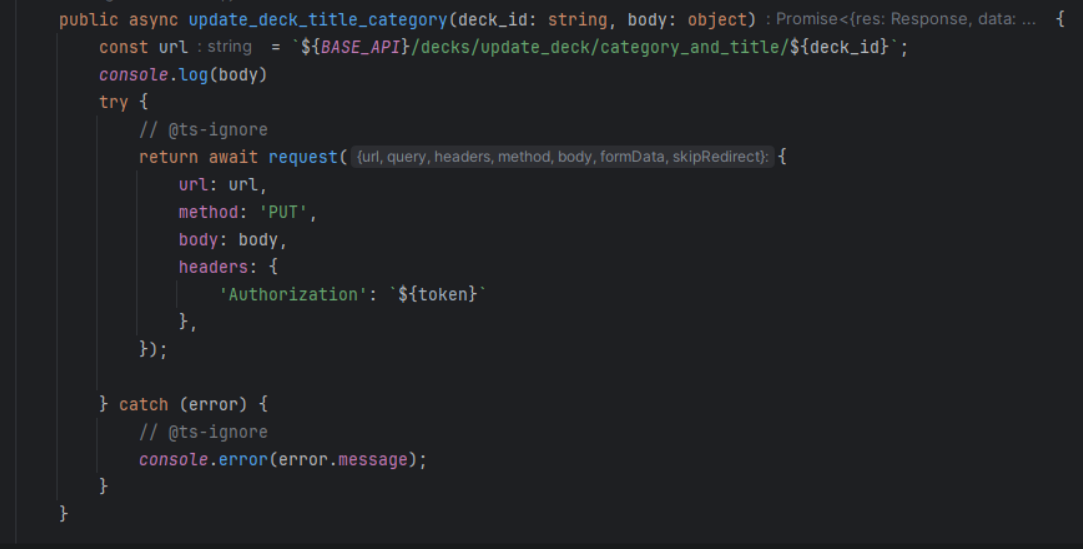
\includegraphics[width=0.7\textwidth]{chapters/chapter_8/screens/update_deck_web}
    \caption{Funkcja służąca do komunikacji z backendowym endpointem do aktualizacji danych talii.}
    \label{img:update_deck_web}
\end{figure}

\begin{figure}[H]
    \centering
    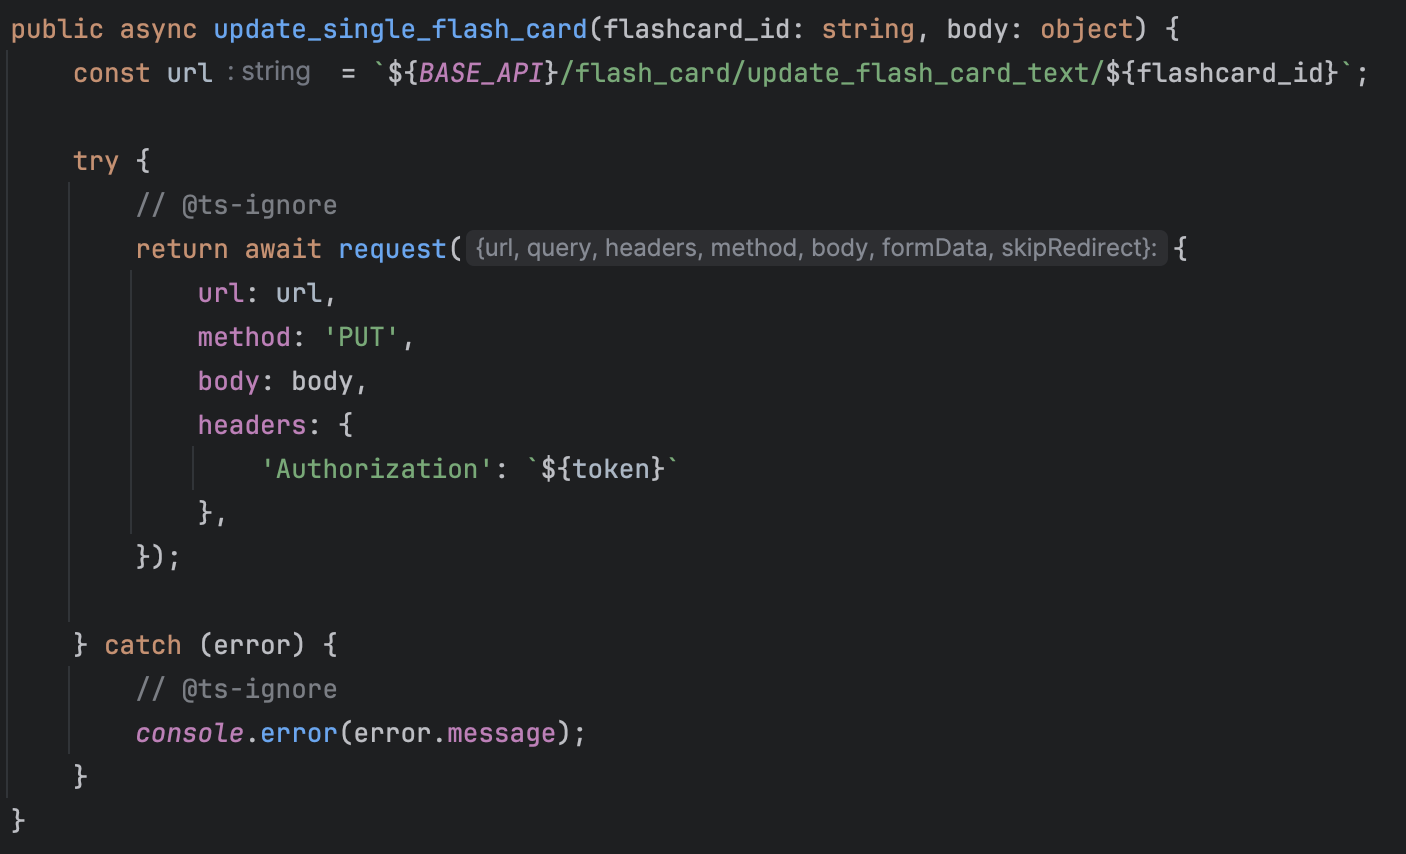
\includegraphics[width=0.7\textwidth]{chapters/chapter_8/screens/update_flash_card_text_web}
    \caption{Funkcja służąca do komunikacji z backendowym endpointem do aktualizacji danych fiszki.}
    \label{img:update_flash_card_web}
\end{figure}

\subsection{Tryb uczenia się z talii fiszek}

\subsubsection{Backend}

Model fiszki zawiera kolumnę \texttt{is\_memorized}, która przy tworzeniu fiszki jest domyślnie ustawiona na "false", wartość ta oznacza, że użytkownika jeszcze nie nauczył się danej treści fiszki. Jeżeli użytkownik uzna, że fiszka została przez niego zapamiętana, to wartość kolumny \texttt{is\_memorized} po zakończonym uczeniu się zostanie zaktualizowana na wartość true. Do aktualizacji danych fiszek została wykorzystany endpoint, który przyjmuje listę fiszek i następnie aktualizuje dane wszystkich fiszek zawartych w przesłanej liście.

\begin{figure}[H]
    \centering
    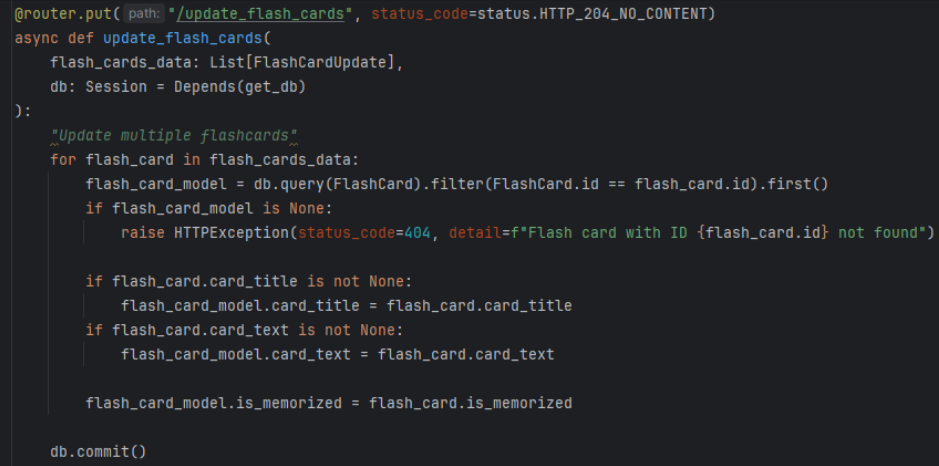
\includegraphics[width=0.7\textwidth]{chapters/chapter_8/screens/update_flash_card_memorized_backend}
    \caption{Logika aktualizacji przesłanych fiszek.}
    \label{img:update_flash_card_memorized_backend}
\end{figure}

\subsubsection{Aplikacja moblina}

Po przejściu do widoku nauki, aplikacja ściąga fiszki użytkownika. W trakcie nauki użytkownik może wybrać dwie opcje "remember" lub "not remember". W momencie kliknięcia przycisku "remember" informacje o fiszce zostaną dodane do listy nauczonych fiszek, które potem zostaną zaktualizowane w bazie. Po zakończeniu nauki, aplikacja ściąga na nowo listę fiszek i filtruje je po polu \texttt{is\_memorized}. Fiszki które mają ustawione \texttt{is\_memorized} na "true", nie zostaną ponownie wyświetlone w trybie nauki.

\begin{figure}[H]
    \centering
    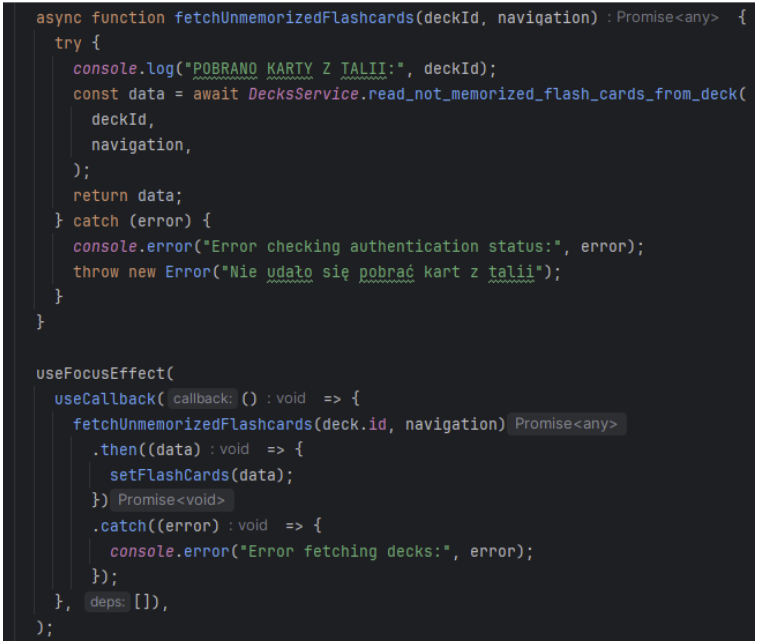
\includegraphics[width=0.7\textwidth]{chapters/chapter_8/screens/get_unmemorized_flash_cards_mobile}
    \caption{Funkcja ściągająca niezapamiętane fiszki.}
    \label{img:get_unmemorized_flash_cards_mobile}
\end{figure}

\begin{figure}[H]
    \centering
    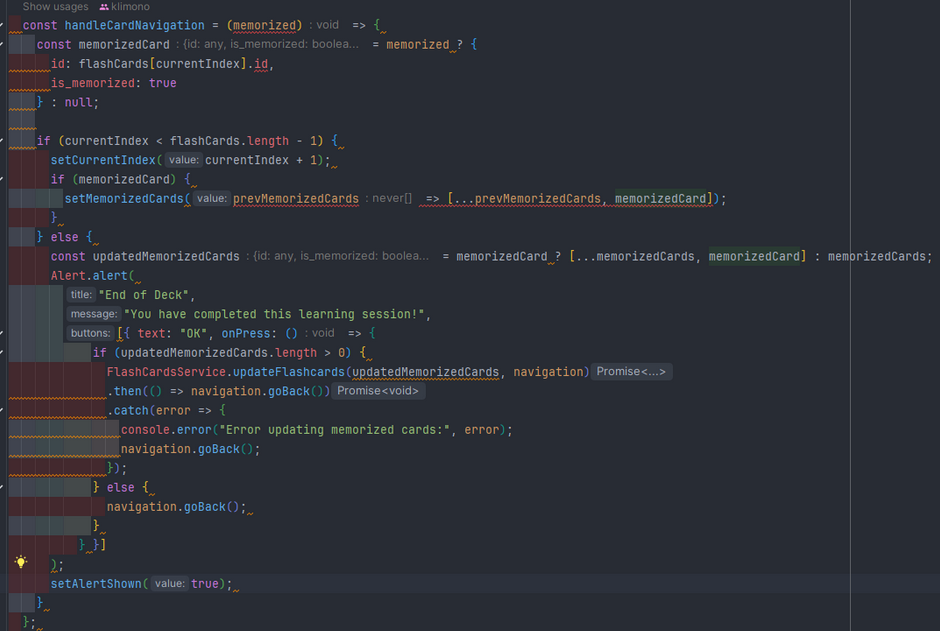
\includegraphics[width=0.7\textwidth]{chapters/chapter_8/screens/update_unmemorized_flash_cards_mobile}
    \caption{Funkcja aktualizacji zapamiętanych fiszek.}
    \label{img:update_unmemorized_flash_cards_mobile}
\end{figure}

\subsubsection{Aplikacja webowe}

Po uruchomieniu trybu uczenia użytkownik widząc fiszkę może kliknąć przycisk "remember" lub "not remember". W przypadku kliknięcia przycisku "remember" informacje o fiszce zostaną dodane do listy fiszek, które zostaną zaktualizowane. Po zakończeniu trybu uczenia list z fiszkami, które zostały oznaczone jako zapamiętane zostaje przekazana do serwisuje, który następnie przekazuje dane do bakcendowego endpointu w celu aktualizacji danych fiszek w bazie danych. Kolumna \texttt{is\_memorized} wszystkich przekazanych fiszek zostaje ustawiona na wartość true. Fiszki, których kolumna \texttt{is\_memorized} jest ustawiona na true nie wyświetlają się w trybie uczenia.

\begin{figure}[H]
    \centering
    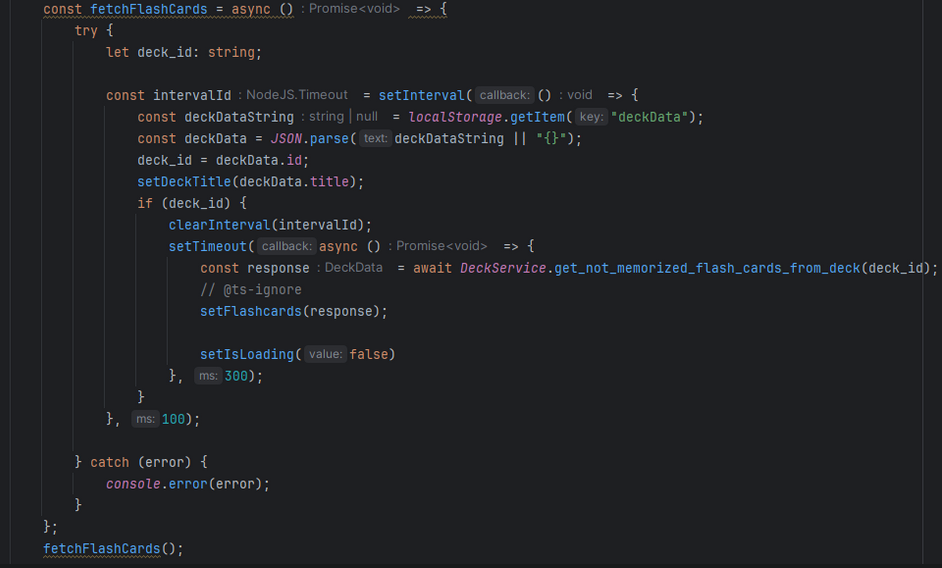
\includegraphics[width=0.7\textwidth]{chapters/chapter_8/screens/get_unmemorized_flash_cards_web}
    \caption{Funkcja ściągająca niezapamiętane fiszki.}
    \label{img:get_unmemorized_flash_cards_web}
\end{figure}

\begin{figure}[H]
    \centering
    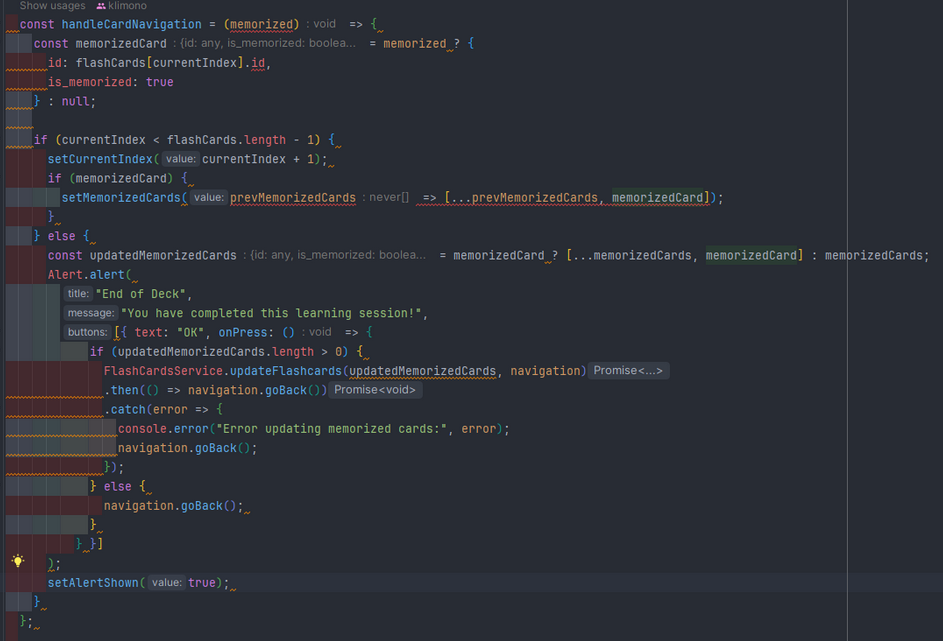
\includegraphics[width=0.7\textwidth]{chapters/chapter_8/screens/pass_unmemorized_flash_cards_web}
    \caption{Funkcja aktualizacji zapamiętanych fiszek.}
    \label{img:pass_unmemorized_flash_cards_web}
\end{figure}

\begin{figure}[H]
    \centering
    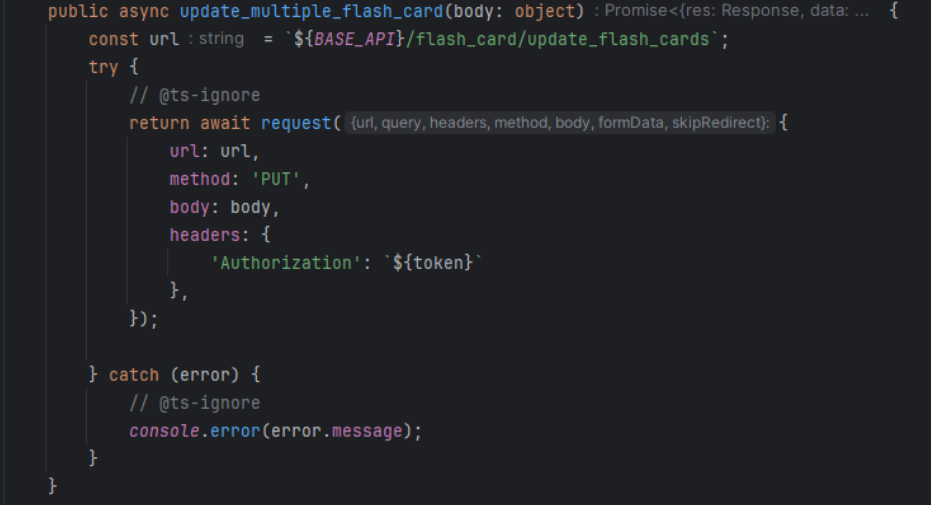
\includegraphics[width=0.7\textwidth]{chapters/chapter_8/screens/update_unmemorized_flash_cards_web}
    \caption{Funkcja aktualizacji zapamiętanych fiszek.}
    \label{img:update_unmemorized_flash_cards_web}
\end{figure}

\subsection{Sterowanie talią przy użyciu mowy}
Funkcjonalność umożliwiająca sterowania talią przy użyciu komend głosowych.


\subsubsection{Backend}
Do wczytania modelu nlp została wykorzystana biblioteka "flair". Do zamiany tekstu na wektory został użyty model "BERT". Została utworzona lista wyrażeń i komend im odpowiadających. Lista ta zostanie  wykorzystana do dopasowania tego co mówi użytkownik do odpowiednich komend głosowych. Funkcja \texttt{vectorize\_text()} odpowiada za konwertowanie tekstu na wektor. Następnie przy użyciu pętli for i funkcji \texttt{vectorize\_text()} zdania w liście są konwertowane na wektory. Następnie została utworzona funkcja \texttt{get\_most\_similar\_answer()}, która przyjmuje zdanie, które wypowiedział użytkownik, i listę wyrażeń. Funkcja ta zmienia zdanie wypowiedziane przez użytkownika na wektor,po czym tworzona jest pustą listę do przechowywania wartości podobieństw pomiędzy wypowiedzią użytkownika a wyrażeniami zawartymi w liście. Pętla for przechodzi po wszystkich wektorach zdań w liście i liczona jest odległość cosinusowa pomiędzy wektorem zdania wypowiedzianego przez użytkownika a wektorem z zdania z listy wyrażeń. Odległość kosinusowa jest używana w analizie tekstu, jest to miara określenia różnicy między dwoma wektorami w przestrzeni n-wymiarowej.\cite{dataMining} Podobieństwo jest liczone ze wzoru 1 - odległość kosinusowa obliczona na podstawie wektora wypowiedzi użytkownika i wektora analizowanego zdania z listy wyrażeń. Obliczone podobieństwo dodawane jest do listy wyrażeń. Następnie przy użyciu \texttt{np.argmax()} zwracany jest indeks na, którym miejscu jest wartość z największym prawdopodobieństwem. Mając indeks funkcja zwraca komendę, która  najbardziej odpowiada zdaniu wypowiedzianemu przez użytkownika. Utworzona została metoda POST, która przyjmuje zdanie wypowiedziane przez użytkownika i uruchamia analizę tekstu.


\begin{figure}[H]
    \centering
    \includegraphics[width=0.7\textwidth]{chapters/chapter_8/screens/backend_nlp}
    \caption{Inicjalizacja modelu wraz z listą wyrażeń i odpowiadających im komend.}
    \label{img:backend_nlp}
\end{figure}


\begin{figure}[H]
    \centering
    \includegraphics[width=0.7\textwidth]{chapters/chapter_8/screens/backend_nlp_usage}
    \caption{Kod odpowiedzialny za analizę tekstu w celu znalezienia najlepiej dopasowanej komendy.}
    \label{img:backend_nlp_usage}
\end{figure}

\subsubsection{Aplikacja mobilna}
Aby obsłużyć głosowy tryb nauki, aplikacja mobilna korzysta z biblioteki "expo-speech” i “expo-av”. Po naciśnięciu przycisku z ikoną mikrofonu aplikacja zaczyna nasłuchiwać komend. Z powodu ograniczeń związanych ze środowiskiem Expo, głos nie jest strumieniowany bezpośrednio do modelu nlp który obsługuje backend. Aplikacja w trakcie nasłuchiwania wykonuje krótkie nagrania, które są tymczasowo zapisywane i wysyłane jako plik audo m4a do backendu. Po ich zinterpretowaniu backend odsyła komendę do której przypisuje znaczenie treści nagrania. Następnie komenda jest wykonywana w widoku nauki.



\begin{figure}[H]
    \centering
    \includegraphics[width=0.7\textwidth]{chapters/chapter_8/screens/mobile_start_recording}
    \caption{Funkcja "startRecording" odpowiedzialna za rozpoczęcie nasłuchiwania.}
    \label{img:mobile_start_recording}
\end{figure}

\begin{figure}[H]
    \centering
    \includegraphics[width=0.7\textwidth]{chapters/chapter_8/screens/mobile_stop_recording}
    \caption{Funkcja "stopRecording" odpowiedzialna za zakończenie nasłuchiwania.}
    \label{img:mobile_stop_recording}
\end{figure}

\begin{figure}[H]
    \centering
    \includegraphics[width=0.7\textwidth]{chapters/chapter_8/screens/mobile_handle_similarity}
    \caption{Funkcja "calculateSimilarity" obsługująca wysłanie nagrania głosowego do modelu nlp.}
    \label{img:mobile_handle_similarity}
\end{figure}

\begin{figure}[H]
    \centering
    \includegraphics[width=0.7\textwidth]{chapters/chapter_8/screens/mobile_handle_voice_commands}
    \caption{Funkcja "handleCommands" obsługująca nawigację w trybie nauki głosowej.}
    \label{img:mobile_handle_voice_commands}
\end{figure}

\subsubsection{Aplikacja webowa}
Do zamiany mowy na tekst, który potem jest analizowany przez model nlp w celu wybrania komendy została wykorzystana biblioteka web speech api. Na początku została utworzona referencja recognition do przechowywania instancji SpeechRecognintion. Po kliknięciu przycisku "start listening" zmienna "isListening" zostaje ustawiona na true rozpoczyna się nasłuchiwanie mowy przy użyciu \texttt{recognition.current.start()}. To co mówi użytkownik jest zapisywane w zmiennej "textControl". Następnie gdy wartość \texttt{textControl} zostaje wypełniona treścią wypowiedzianą przez użytkownika zostanie to przekazane do funkcji \texttt{nlpModelControl()}. Funkcja ta wysyła wypowiedź użytkownika do modelu nlp na backendzie, model nlp analizy treści i dopasowuje  zdanie, które jest najbliższe semantycznie do wypowiedzi użytkownika. Następnie sprawdzana jest komenda,która przypisana jest do wybranego zdania. Komenda zostaje przesłana na frontend i przekazana do funkcji \texttt{voiceControl()}, która zawiera switch case, przesłana komenda uruchamia odpowiednią akcję na stronie internetowej.


\begin{figure}[H]
    \centering
    \includegraphics[width=0.7\textwidth]{chapters/chapter_8/screens/recognition_reference}
    \caption{Referencja "recognition".}
    \label{img:recognition_reference}
\end{figure}


\begin{figure}[H]
    \centering
    \includegraphics[width=0.7\textwidth]{chapters/chapter_8/screens/begin_listening}
    \caption{Rozpoczęcie nasłuchiwania.}
    \label{img:begin_listening}
\end{figure}

\begin{figure}[H]
    \centering
    \includegraphics[width=0.7\textwidth]{chapters/chapter_8/screens/textControl_write}
    \caption{Zapisywanie tego co mówi użytkownik do zmiennej "textControl".}
    \label{img:textControl_write}
\end{figure}



\begin{figure}[H]
    \centering
    \includegraphics[width=0.7\textwidth]{chapters/chapter_8/screens/textControl_to_nlp}
    \caption{Przekazanie zawartości textControl do "nlpModelControl".}
    \label{img:textControl_to_nlp}
\end{figure}

\begin{figure}[H]
    \centering
    \includegraphics[width=0.7\textwidth]{chapters/chapter_8/screens/nlp_to_voiceControl}
    \caption{Komenda wybrana przez model nlp zostaje przekazana do "voiceControl()".}
    \label{img:nlp_to_voiceControl}
\end{figure}

\begin{figure}[H]
    \centering
    \includegraphics[width=0.7\textwidth]{chapters/chapter_8/screens/sent_message}
    \caption{Funkcja "sent\_message()" przekazuje wypowiedź użytkownika do modelu nlp na backendzie.}
    \label{img:sent_message}
\end{figure}

\begin{figure}[H]
    \centering
    \includegraphics[width=0.7\textwidth]{chapters/chapter_8/screens/voice_control_web}
    \caption{Na podstawie otrzymanej komendy aplikacja wykonuje odpowiednią akcję.}
    \label{img:voice_control_web}
\end{figure}

\subsection{Import talii innych użytkowników}
Funkcjonalność pozwalająca użytkownikom na zapisanie talii udostępnionej publicznie.

\subsubsection{Backend}
Utworzona została metoda POST, która służy do kopiowania talii innych użytkowników. Przyjmuje ona identyfikator talii do skopiowania i identyfikator użytkownika, który tę talię chce zaimportować. Metoda tworzy nową niezależna talią, która zostaje przypisana do użytkownika o podanym identyfikatorze. Pozycje w rankingu talii są przyznawane na podstawie liczby pobrań, natomiast pozycja w rankingu jest zależna od sumy pobrań wszystkich jego udostępnionych talii. Użytkownik ma teraz możliwość importowania talii fiszek. Pobrana talia zostaje dodana do widoku public decs.

\begin{figure}[H]
    \centering
    \includegraphics[width=0.7\textwidth]{chapters/chapter_8/screens/backend_copy_deck}
    \caption{Metoda POST do kopiowania talii.}
    \label{img:backend_copy_deck}
\end{figure}

\subsubsection{Aplikacja mobilna}
Funkcja przekazuje do serwisu dane, takie jak identyfikator wybranej talii oraz identyfikator użytkownika, następnie wysyła request na api, aby dodać wybraną talię do listy użytkownika.

\begin{figure}[H]
    \centering
    \includegraphics[width=0.7\textwidth]{chapters/chapter_8/screens/mobile_download_deck}
    \caption{Funkcja obsługująca pobranie publicznej talii.}
    \label{img:mobile_download_deck}
\end{figure}

\begin{figure}[H]
    \centering
    \includegraphics[width=0.7\textwidth]{chapters/chapter_8/screens/mobile_deck_download_service}
    \caption{Funkcja odpowiedzialna za pobieranie / kopiowanie talii.}
    \label{img:mobile_deck_download_service}
\end{figure}

\subsubsection{Aplikacja webowa}
Użytkownik żeby zaimportować talie musi kliknąć w przycisk "Import deck". Po kliknięciu w przycisk z pamięci lokalnej zostaje pobrany identyfikator talii i użytkownika. Te informacje zostają przekazane do serwisu, który łączy się z endpointem na backendzie i przekazuje dane talii i użytkownika potrzebne do skopiowania talii fiszek.

\begin{figure}[H]
    \centering
    \includegraphics[width=0.7\textwidth]{chapters/chapter_8/screens/web_download_deck}
    \caption{Funkcja odpowiedzialna za aktywację serwisu do kopiowania talii.}
    \label{img:web_download_deck}
\end{figure}

\begin{figure}[H]
    \centering
    \includegraphics[width=0.7\textwidth]{chapters/chapter_8/screens/web_service_download_deck}
    \caption{Service do łączenia się z metodą "copy\_deck" na backendzie.}
    \label{img:web_service_download_deck}
\end{figure}

\subsection{Tryb dark mode i light mode}
Funkcjonalność umożliwiająca zmianę stylu aplikacji na jasny lub ciemny. Zaimplementowana tylko w aplikacji mobilnej bez konieczności nawiązywania połączenia z backendem.

\subsubsection{Aplikacja moblina}
Przycisk do zmiany motywu został dodany do panelu użytkownika w sekcji ustawienia. Działanie jest proste, po kliknięciu następuje zmiana trybu na przeciwny. W zależności od aktywnego motywu, zmienia się ikona przycisku.

\begin{figure}[H]
    \centering
    \includegraphics[width=0.7\textwidth]{chapters/chapter_8/screens/darkmode}
    \caption{Implementacja i wywołanie przycisku zmieniającego motyw aplikacji na ciemny.}
    \label{img:darkmode}
\end{figure}

\subsection{Generowanie treści fiszki na podstawie słów kluczowych}
Funkcjonalność, która pozwala na wygenerowanie treści fiszki używając ChatGPT.

\subsubsection{Backend}
Do generowania treści zostało wykorzystane api ChatGPT. Została utworzona metoda POST, która pozwala na wysłanie tekstu do endpointu. Na podstawie otrzymanej treści ChatGPT generuje treść i odsyła ją do aplikacji. Klucz api trzymany jest w zmiennych środowiskowych.

\begin{figure}[H]
    \centering
    \includegraphics[width=0.7\textwidth]{chapters/chapter_8/screens/backend_chat}
    \caption{Endpoint służący do komunikacji z ChatGPT.}
    \label{img:backend_chat}
\end{figure}

\subsubsection{Aplikacja mobilna}
Aby wygenerować definicje fiszki z ChatGPT, użytkownik musi mieć wypełniony tytuł fiszki. Następnie funkcja wysyła na wstakany endpoint tytuł fiszki, API kontaktuje się z ChatGPT w celu wygenerowania definicji. Bo wygenerowaniu definicji, zostaje ona zwrócona na front, gdzie wartość definicji zostaje nadpisana. Następnie po zatwierdzeniu fiszki przez użytkownika, aplikacja wysyła dane na api gdzie zostaje utworzona fiszka dla edytowanej talii.

\begin{figure}[H]
    \centering
    \includegraphics[width=0.7\textwidth]{chapters/chapter_8/screens/mobile_chat}
    \caption{Funkcja obsługująca generowanie treści za pomocą ChatGPT.}
    \label{img:mobile_chat_1}
\end{figure}

\subsubsection{Aplikacja webowa}
Został utworzony service, który pozwala na połączenie z bakcendowym endpointem do komunikacji z api ChatGPT. Aby treść fiszki została wygenerowana użytkownik musi na przedniej stronie fiszki napisać wiadomość i kliknąć przycisk generate. Po kliknięciu treść z przedniej strony fiszki zostaje przekazana do funkcji, która wysyła pobraną treść do backendowego endpointu, następnie ChatGPT na podstawie otrzymanego kontentu generuje odpowiedź. Po otrzymaniu odpowiedzi na stronie webowej wyskakuje okienko z informacją, że treści generowane przez ChatGPT mogą być nieprawdziwe, poniżej znajduje się wygenerowana wiadomość, użytkownik może zaakceptować otrzymana treść lub nie. W przypadku jeżeli zaakceptuje wiadomość tylna strona fiszki zostanie zapełniona wygenerowaną wiadomością w przeciwnym wypadku fiszka zostaje pusta.

\begin{figure}[H]
    \centering
    \includegraphics[width=0.7\textwidth]{chapters/chapter_8/screens/web_chat_1}
    \caption{Funkcja, która pobiera treść fiszki z przedniej strony karty i przekazuje wiadomośc do service odpowiedzialnego za komunikację z backendem.}
    \label{img:web_chat_1}
\end{figure}

\begin{figure}[H]
    \centering
    \includegraphics[width=0.7\textwidth]{chapters/chapter_8/screens/web_chat_2}
    \caption{Funkcja służąca do komunikacji backendowym endpointem do wysyłania wiadomości do ChatGPT.}
    \label{img:web_chat_2}
\end{figure}